Careful analysis of the mathematical models above leads us to identify several important factors that influence the quality of an application's execution using Lazy Shadowing. These factors can be classified into three categories, i.e., system category, application category, and Lazy Shadowing category. The system category includes static power ratio, $\rho$ ($\rho=p_s/p$), and MTBF of each core; the application category is mainly the total workload, $W$; and Lazy Shadowing category involves the number of cores to use, $N$, and shadowing ratio, $\alpha$, which together determine the number of main cores and shadow cores ($N=M+S$ and $\alpha=M/S$). In this section, we evaluate each performance metric of Lazy Shadowing, 
 %using the models above, 
 with the influence of each of the factors considered. %First we calculate the application failure probability for various scenarios. Then we proceed to study the expected energy consumption and completion time under different application failure probabilities. 

%\subsection{Application failure probability}
%\label{eval_app_fail_prob}
%\input{Evaluation/app_fail_prob}

%\subsection{Comparison to process replication}
%\label{eval_comparison}
%%To study the performance of Lazy Shadowing, we compare with process replication using the analytical models in Section~\ref{sec:analytical}. We also compare to checkpointing, of which the completion time is calculated with Daly's model~\cite{daly_fgcs_2006} and the energy consumption is then derived using Equation~\ref{eq:exp_energy1}. 
We compare with both process replication and checkpointing, assuming the same number of cores to use. The completion time with checkpointing is calculated with Daly's model~\cite{daly_fgcs_2006} assuming 10 minutes for both checkpointing and restart. The energy consumption is then derived with Equation~\ref{eq:exp_energy1}. It is important to point out that we always assume the same number of cores. 


It is clear from THEOREM 1 that the total recovery delay $\sum_{i=1}^k\tau_i$ is determined by the execution time $\sum_{i=1}^k\Delta_i$, independent of the distribution of failures. 
% which determines the individual value of $\Delta_i$. 
Therefore, our models are generic with no assumption about failure probability distribution, and the expectation of the total delay from all failures is the same as if failures are uniformly distributed~\cite{daly_fgcs_2006}. Specifically, $\Delta_i = w/(k+1)$, and $T_c^k = w + w*(1-\sigma_s^b)*\frac{k}{k+1}$. Further, we assume that each shadow gets a fair share of its core's execution rate so that $\sigma_s^b = \frac{1}{\alpha}$. %One may argue that the execution rate of the shadows
%should be degraded because of increased memory pressure or communication overhead. %Agreeing with that, however, we argue that 
%time sharing, which is the basic mechanism of multi-programming OS, is able to overlap computation and communication and improve system efficiency. For completeness, though, 
%To take that into account, we have also studied the slowing down effect using a penalty model, to be discussed later. 
To calculate Equation~\ref{eq:exp_energy2}, we assume that the dynamic power during shadow leaping is twice of that during normal execution, i.e., $p_{l}=2*p_d$, and the time for shadow leaping through RDMA is half of the recovery time, i.e., $T_l=0.5*(T_{total} - w)$. %The static power ratio $\rho$ is fixed at 0.5 for our first study, other values are also studied in this section.

The first study uses $N=1$ million cores, %effectively simulating the future extreme-scale computing environment, and assumes that $W=1$ million hours. 
$W=1$ million hours, and static power ratio $\rho=0.5$.
For Lazy Shadowing we vary $\alpha$ from 1 to 10, understanding that it is unrealistic to collocate too many processes on a core. Besides $\alpha=1$, which is process replication, we only show $\alpha=5$ and $\alpha=10$ as others can be easily inferred from the figures.

\begin{figure}[!t]
	\begin{center}
%		\subfigure[application fatal failure probability]
%		{
%			\label{fig:f3}
%			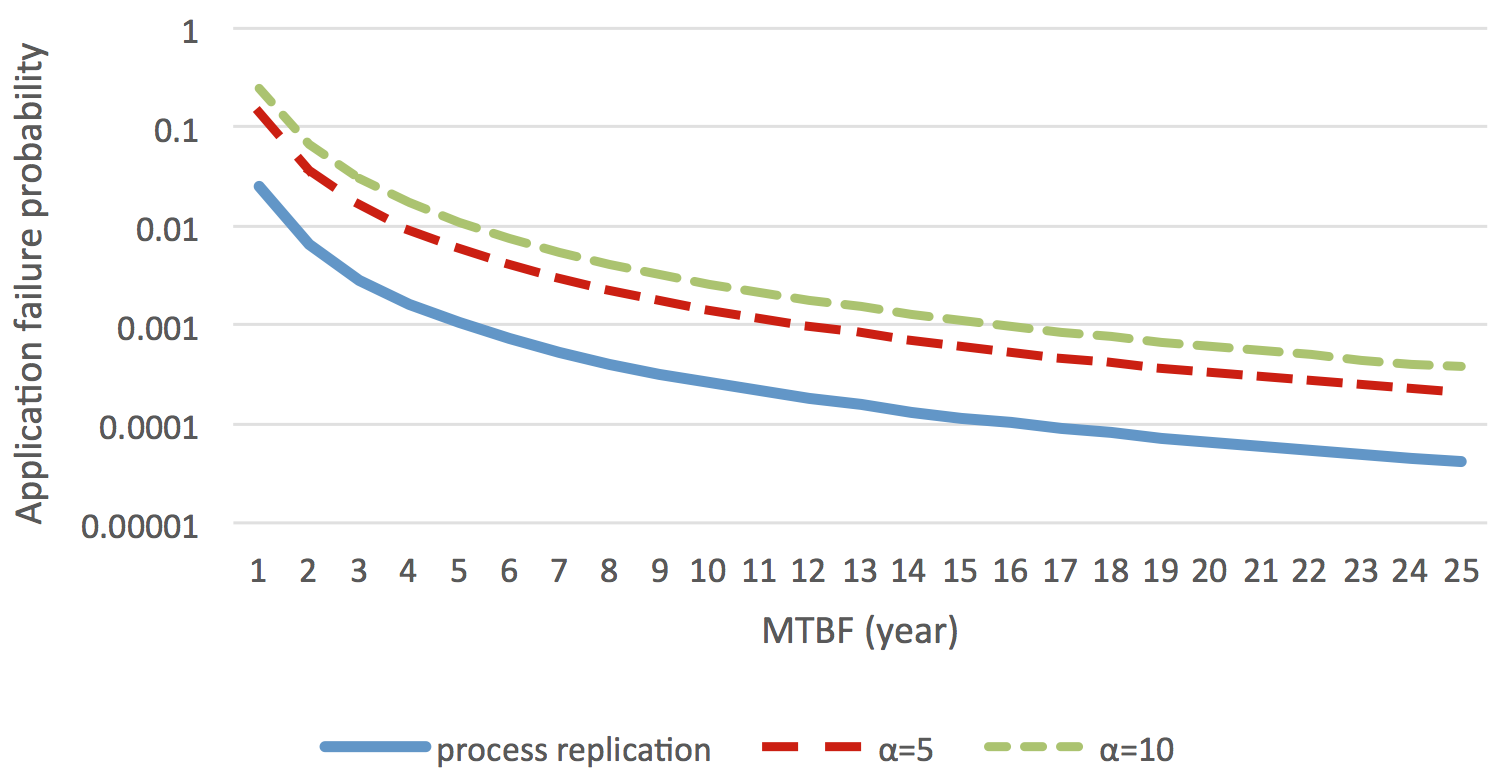
\includegraphics[width=0.7\columnwidth]{Figures/f3}
%		} 
%		\subfigure[Expected completion time]
%		{
%			\label{fig:t31}
%			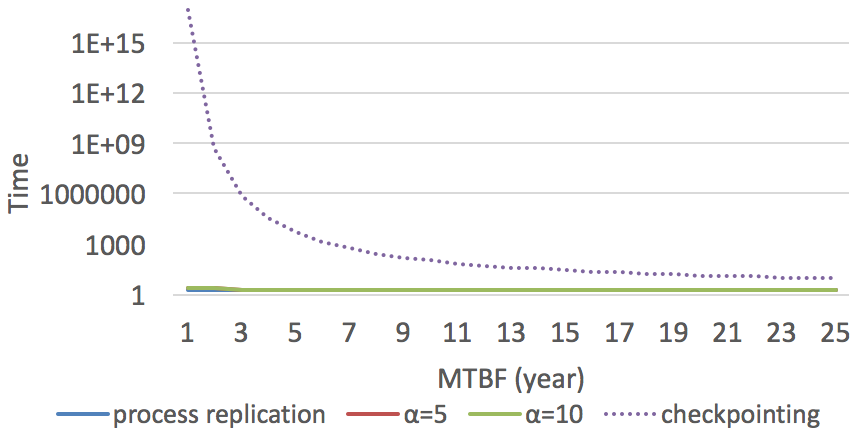
\includegraphics[width=0.7\columnwidth]{Figures/tt31}
%		} 
		\subfigure[Expected completion time]
		{
			\label{fig:t32}
			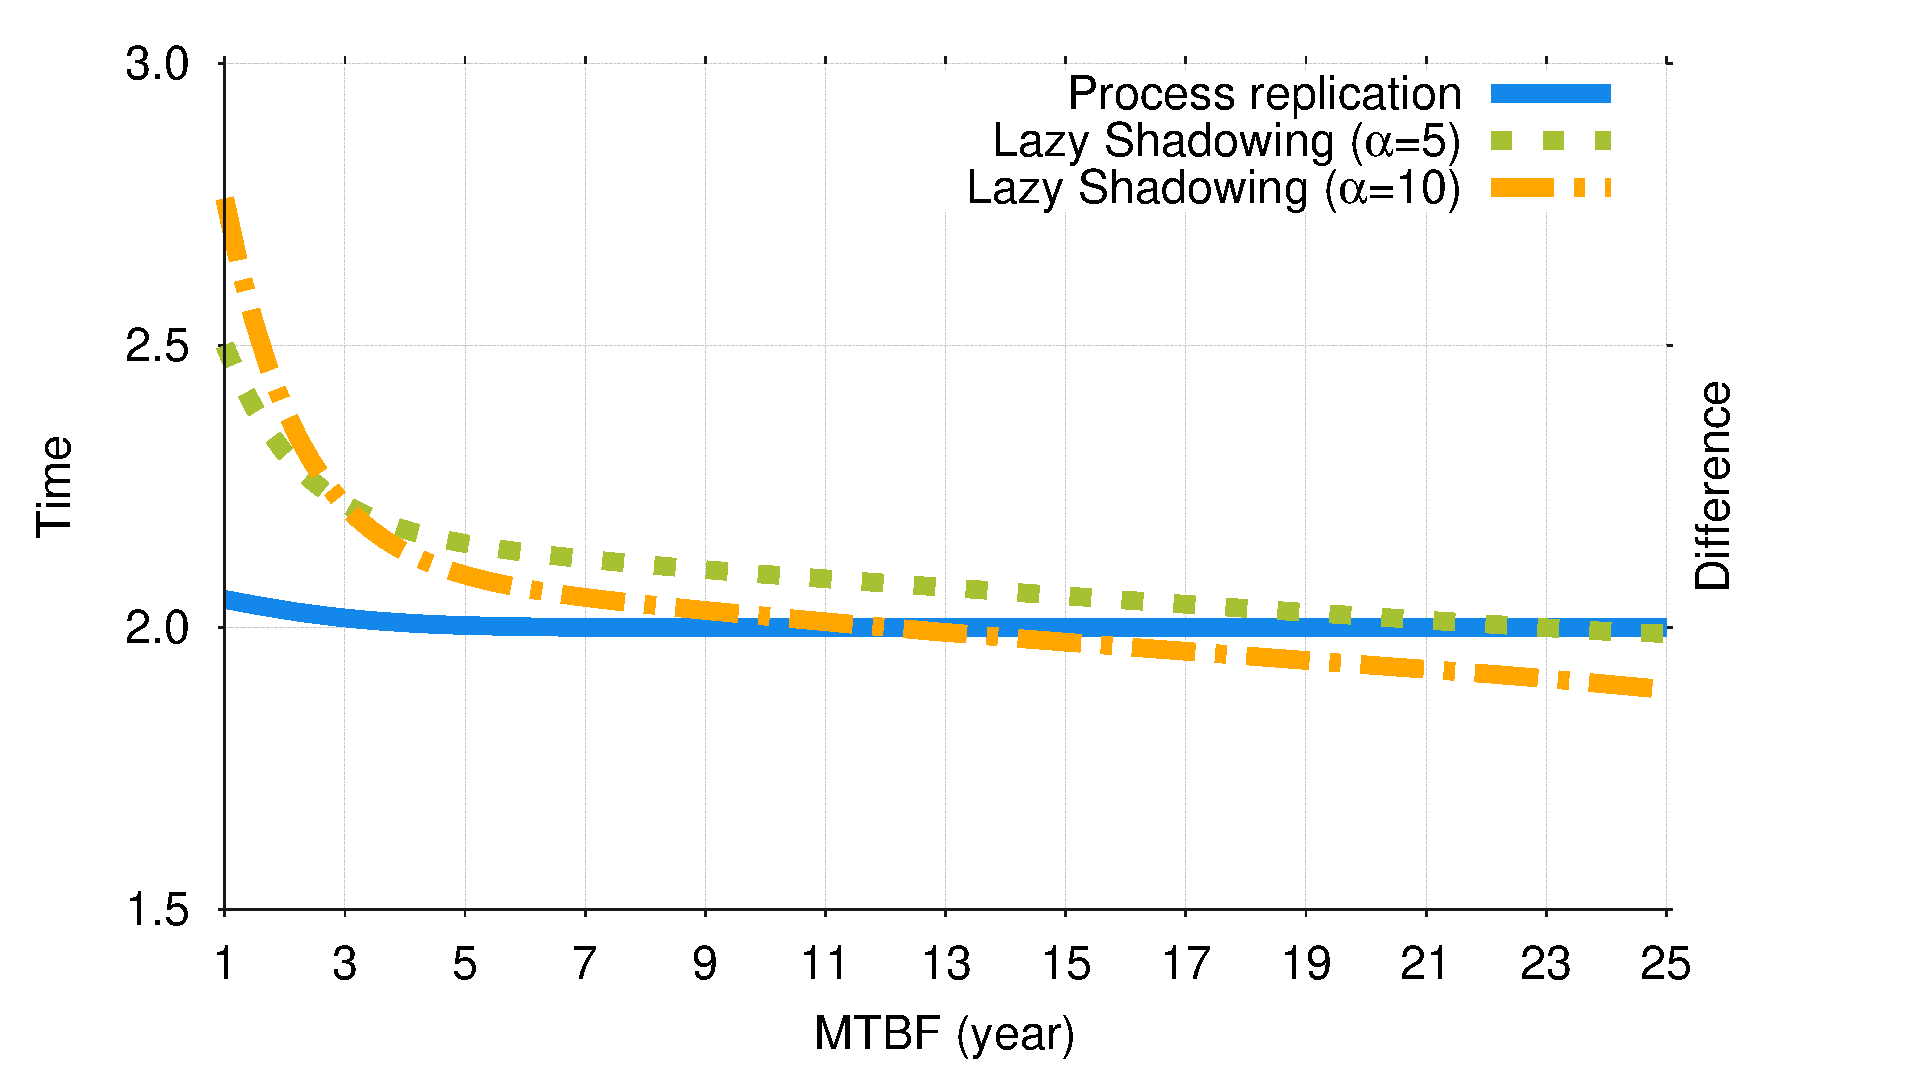
\includegraphics[width=0.7\columnwidth]{Figures/gen_time.eps}
			%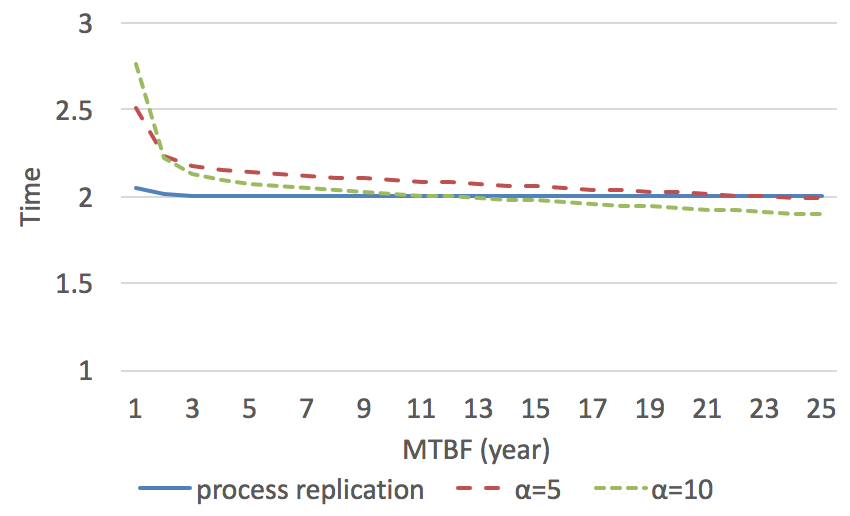
\includegraphics[width=0.7\columnwidth]{Figures/tt32}
		} 
		\subfigure[Expected energy consumption]
		{
			\label{fig:e32}
			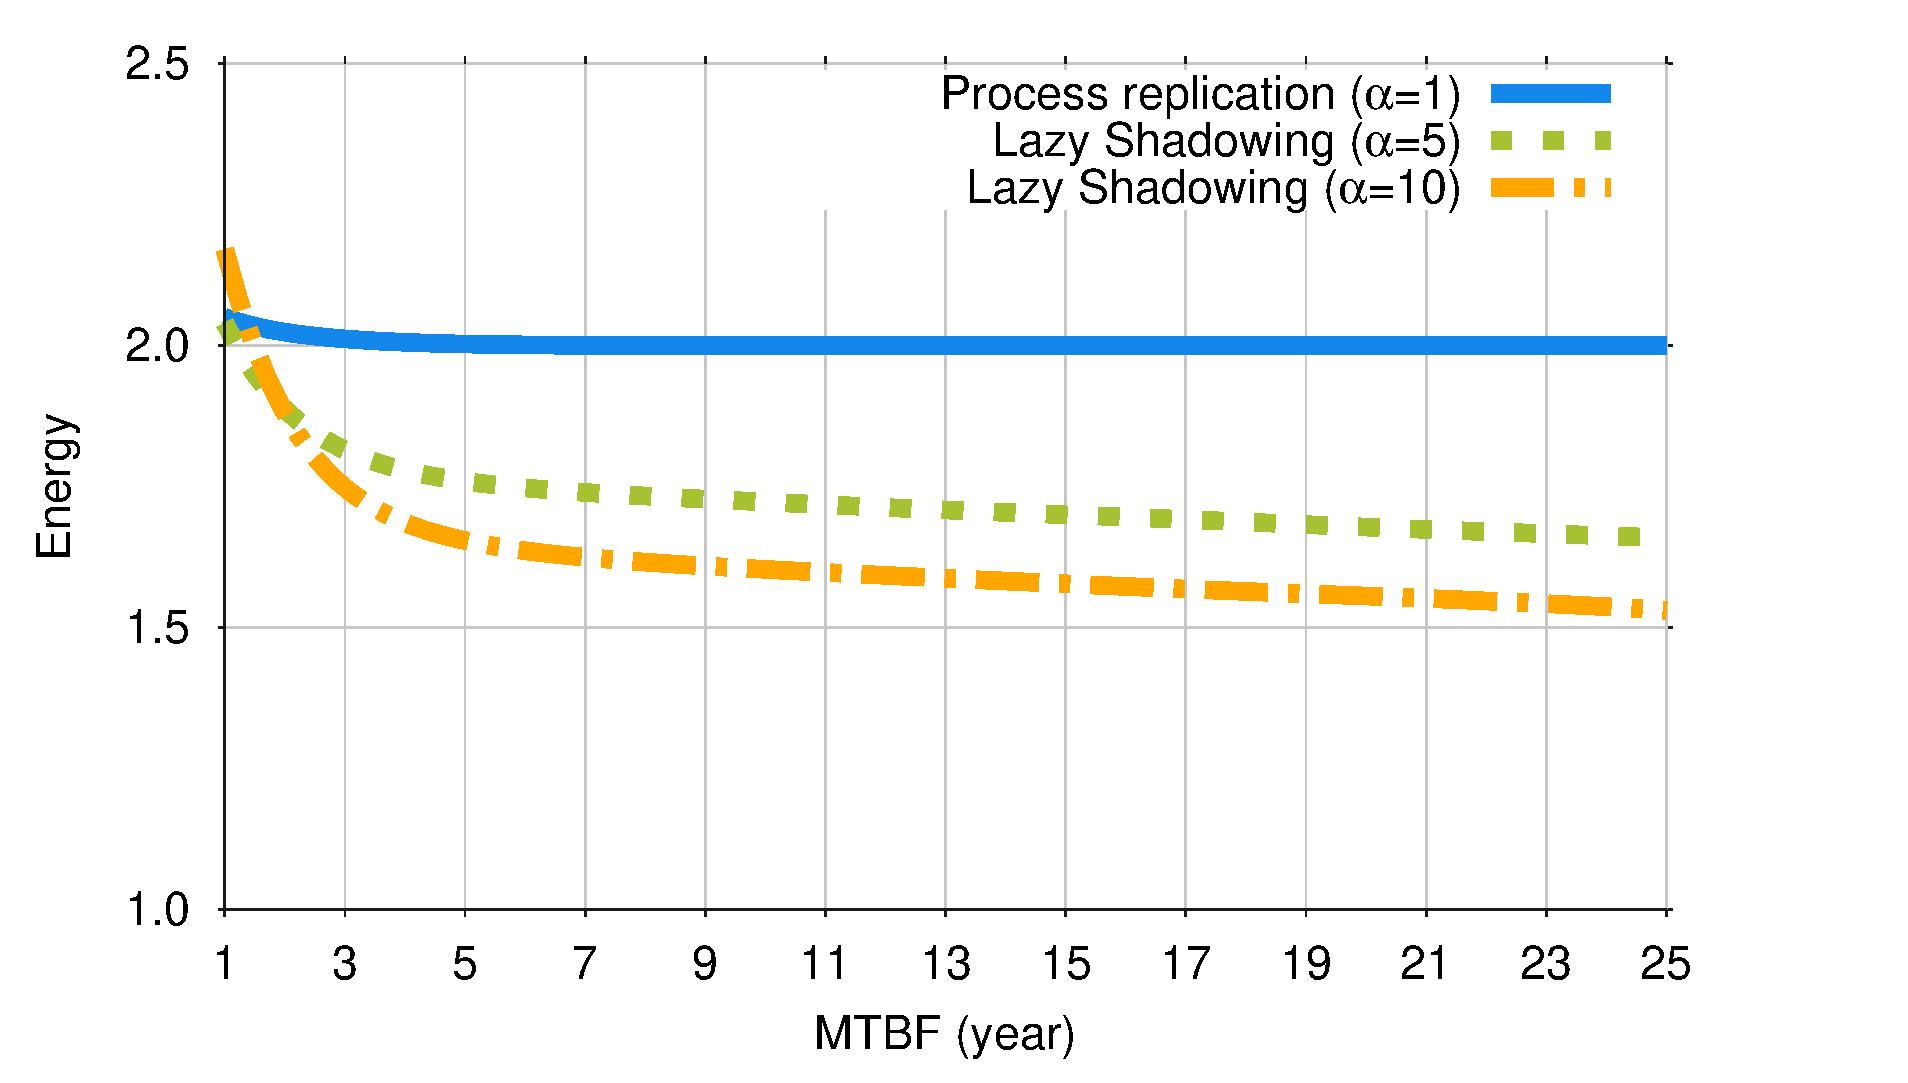
\includegraphics[width=0.7\columnwidth]{Figures/gen_energy.eps}
			%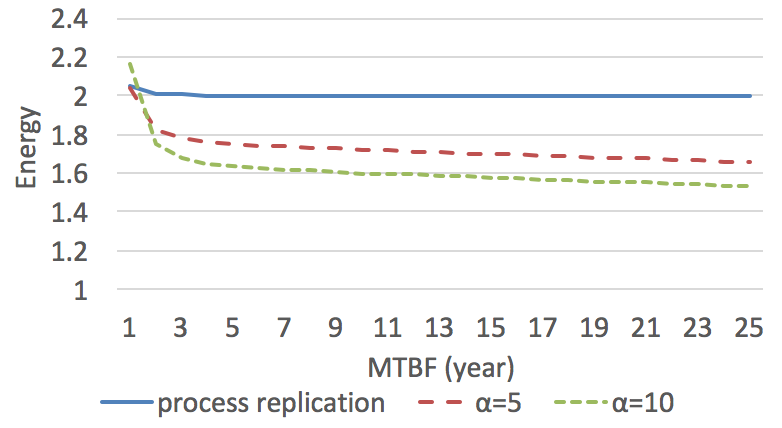
\includegraphics[width=0.7\columnwidth]{Figures/te32}
		} 
	\end{center}
	%\vskip -0.22in 
	\caption{Comparison of completion time and energy consumption. $W=10^6$ hours, $N=10^6$, $\rho=0.5$.}
	\label{fig:3}
\end{figure}

%By definition, the application fatal failure probability for checkpointing is 0, as it periodically saves the execution states, from which the computation can be resumed upon failure. Figure~\ref{fig:f3} shows that due to collocation, the application fatal failure probability increases for Lazy Shadowing. 
We had a comprehensive study of the application fatal failure probabilities using models in Section~\ref{anal_app_fail}. Results show that application fatal failure probability increases slightly for Lazy Shadowing compared to process replication, as a result of shadow collocation (discussed in Section~\ref{sec:leaping_shadows}). However, even with unrealistically low MTBF of 1 year, Lazy Shadowing is still able to complete without rollback with greater than 0.75 probability. Therefore, we will not further discuss application fatal failure probability.  


%It is clear from Figure~\ref{fig:t31} that checkpointing incurs significant delay, indicating that it may not be a viable fault tolerance approach for future extreme-scale computing. 
Our results show that at extreme-scale, the completion time and energy consumption of checkpointing are orders of magnitude larger than those of Lazy Shadowing and process replication. Thus, we choose not to plot a separate graph for checkpointing in the interest of space. 
%so large that the comparison between process replication and Lazy Shadowing is invisible. Therefore, we re-plot the comparison between Lazy Shadowing and process replication in Figure~\ref{fig:t32} and~\ref{fig:e32}, with checkpointing removed. 
Figure~\ref{fig:t32} reveals that the most time efficient choice largely depends on MTBF. 
%More specifically, process replication consumes less time when MTBF is low while otherwise Lazy Shadowing is more efficient.
When MTBF is high, Lazy Shadowing requires less time as more cores are used for main processes and less workload is assigned to each process. As MTBF decreases, process replication outperforms Lazy Shadowing as a result of the increased likelyhood of rollback for Lazy Shadowing.
%This is because of the increased probability of re-execution for Lazy Shadowing when failure rate is high. 
In terms of energy consumption, Lazy Shadowing has much more advantage over process replication. For MTBF from 2 to 25 years, Lazy Shadowing with $\alpha=5$ can achieve 9.6-17.1\% energy saving, while the saving increases to 13.1- 23.3\% for $\alpha=10$. The only exception is when MTBF is extremely low (1 year), Lazy Shadowing with $\alpha=10$ consumes more energy because of extended execution time.








%\subsection{Energy comparison}
%\label{eval_energy_comp}
%\input{Evaluation/energy_comp}

\subsection{Comparison to checkpointing and process replication}
\label{eval_comparison}
%To study the performance of Lazy Shadowing, we compare with process replication using the analytical models in Section~\ref{sec:analytical}. We also compare to checkpointing, of which the completion time is calculated with Daly's model~\cite{daly_fgcs_2006} and the energy consumption is then derived using Equation~\ref{eq:exp_energy1}. 
We compare with both process replication and checkpointing, assuming the same number of cores to use. The completion time with checkpointing is calculated with Daly's model~\cite{daly_fgcs_2006} assuming 10 minutes for both checkpointing and restart. The energy consumption is then derived with Equation~\ref{eq:exp_energy1}. It is important to point out that we always assume the same number of cores. 


It is clear from THEOREM 1 that the total recovery delay $\sum_{i=1}^k\tau_i$ is determined by the execution time $\sum_{i=1}^k\Delta_i$, independent of the distribution of failures. 
% which determines the individual value of $\Delta_i$. 
Therefore, our models are generic with no assumption about failure probability distribution, and the expectation of the total delay from all failures is the same as if failures are uniformly distributed~\cite{daly_fgcs_2006}. Specifically, $\Delta_i = w/(k+1)$, and $T_c^k = w + w*(1-\sigma_s^b)*\frac{k}{k+1}$. Further, we assume that each shadow gets a fair share of its core's execution rate so that $\sigma_s^b = \frac{1}{\alpha}$. %One may argue that the execution rate of the shadows
%should be degraded because of increased memory pressure or communication overhead. %Agreeing with that, however, we argue that 
%time sharing, which is the basic mechanism of multi-programming OS, is able to overlap computation and communication and improve system efficiency. For completeness, though, 
%To take that into account, we have also studied the slowing down effect using a penalty model, to be discussed later. 
To calculate Equation~\ref{eq:exp_energy2}, we assume that the dynamic power during shadow leaping is twice of that during normal execution, i.e., $p_{l}=2*p_d$, and the time for shadow leaping through RDMA is half of the recovery time, i.e., $T_l=0.5*(T_{total} - w)$. %The static power ratio $\rho$ is fixed at 0.5 for our first study, other values are also studied in this section.

The first study uses $N=1$ million cores, %effectively simulating the future extreme-scale computing environment, and assumes that $W=1$ million hours. 
$W=1$ million hours, and static power ratio $\rho=0.5$.
For Lazy Shadowing we vary $\alpha$ from 1 to 10, understanding that it is unrealistic to collocate too many processes on a core. Besides $\alpha=1$, which is process replication, we only show $\alpha=5$ and $\alpha=10$ as others can be easily inferred from the figures.

\begin{figure}[!t]
	\begin{center}
%		\subfigure[application fatal failure probability]
%		{
%			\label{fig:f3}
%			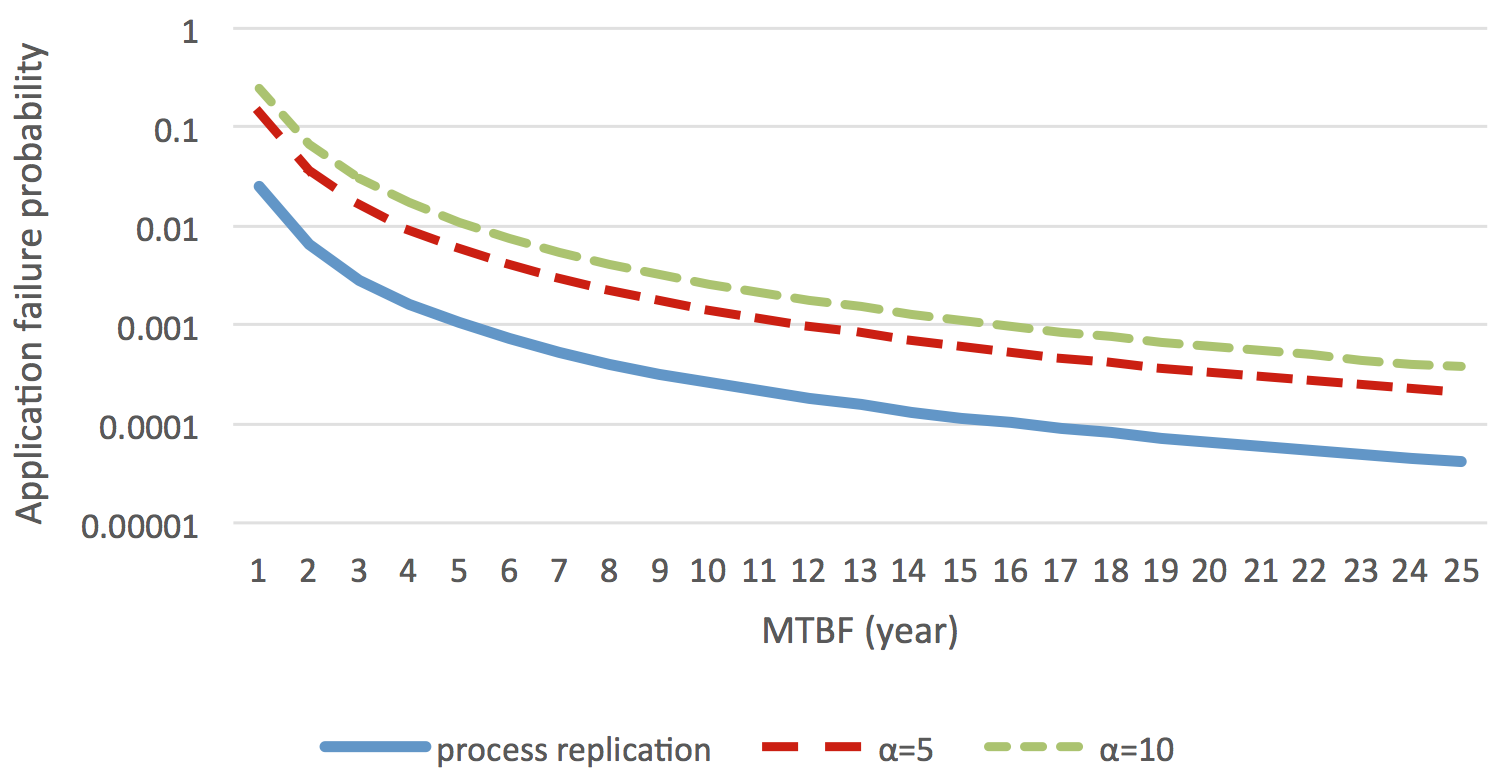
\includegraphics[width=0.7\columnwidth]{Figures/f3}
%		} 
%		\subfigure[Expected completion time]
%		{
%			\label{fig:t31}
%			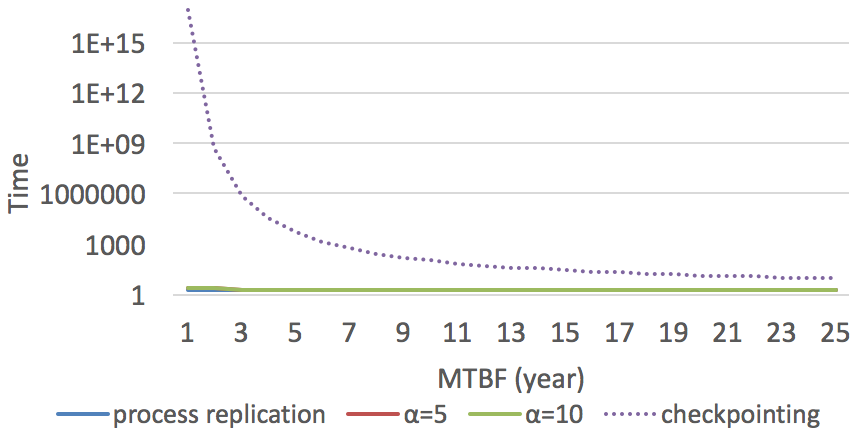
\includegraphics[width=0.7\columnwidth]{Figures/tt31}
%		} 
		\subfigure[Expected completion time]
		{
			\label{fig:t32}
			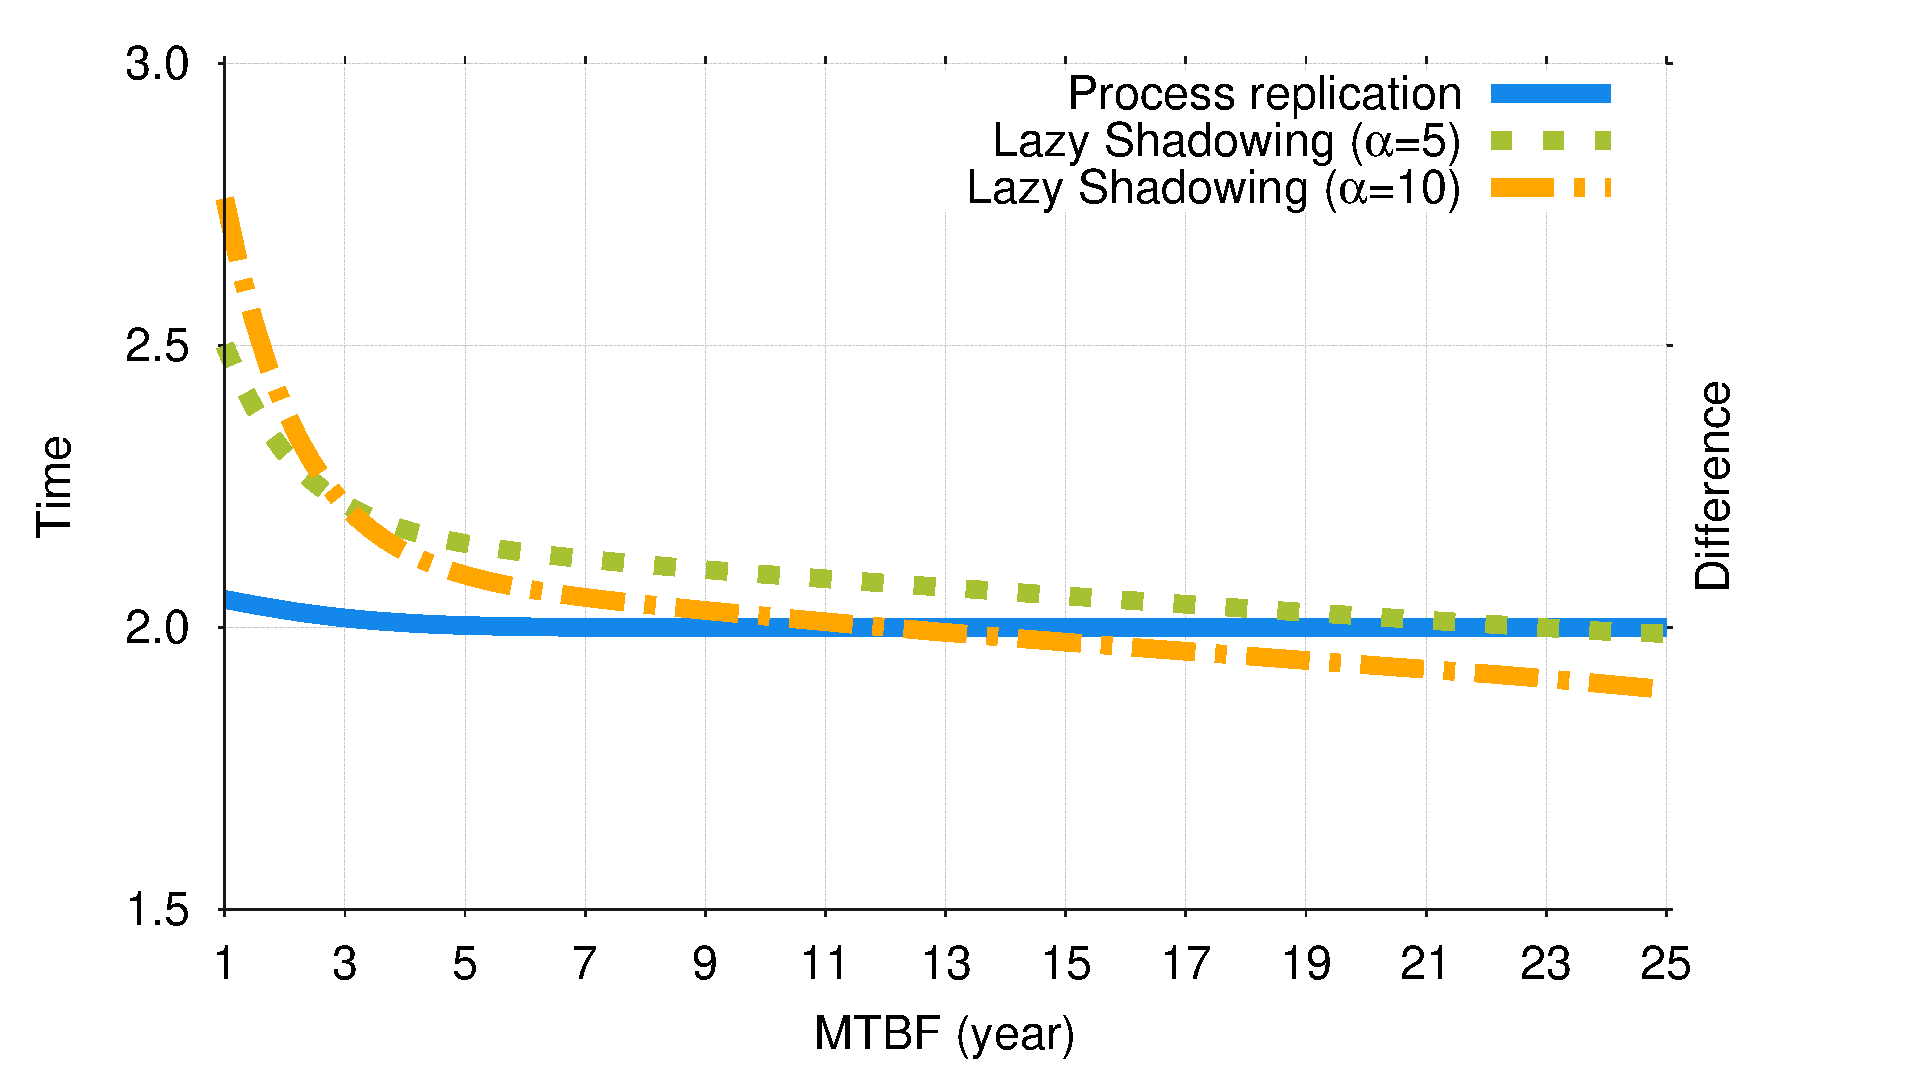
\includegraphics[width=0.7\columnwidth]{Figures/gen_time.eps}
			%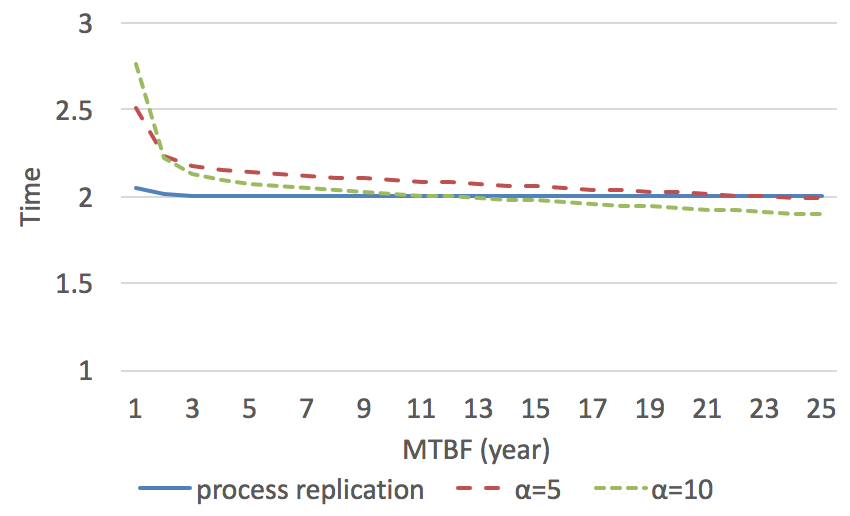
\includegraphics[width=0.7\columnwidth]{Figures/tt32}
		} 
		\subfigure[Expected energy consumption]
		{
			\label{fig:e32}
			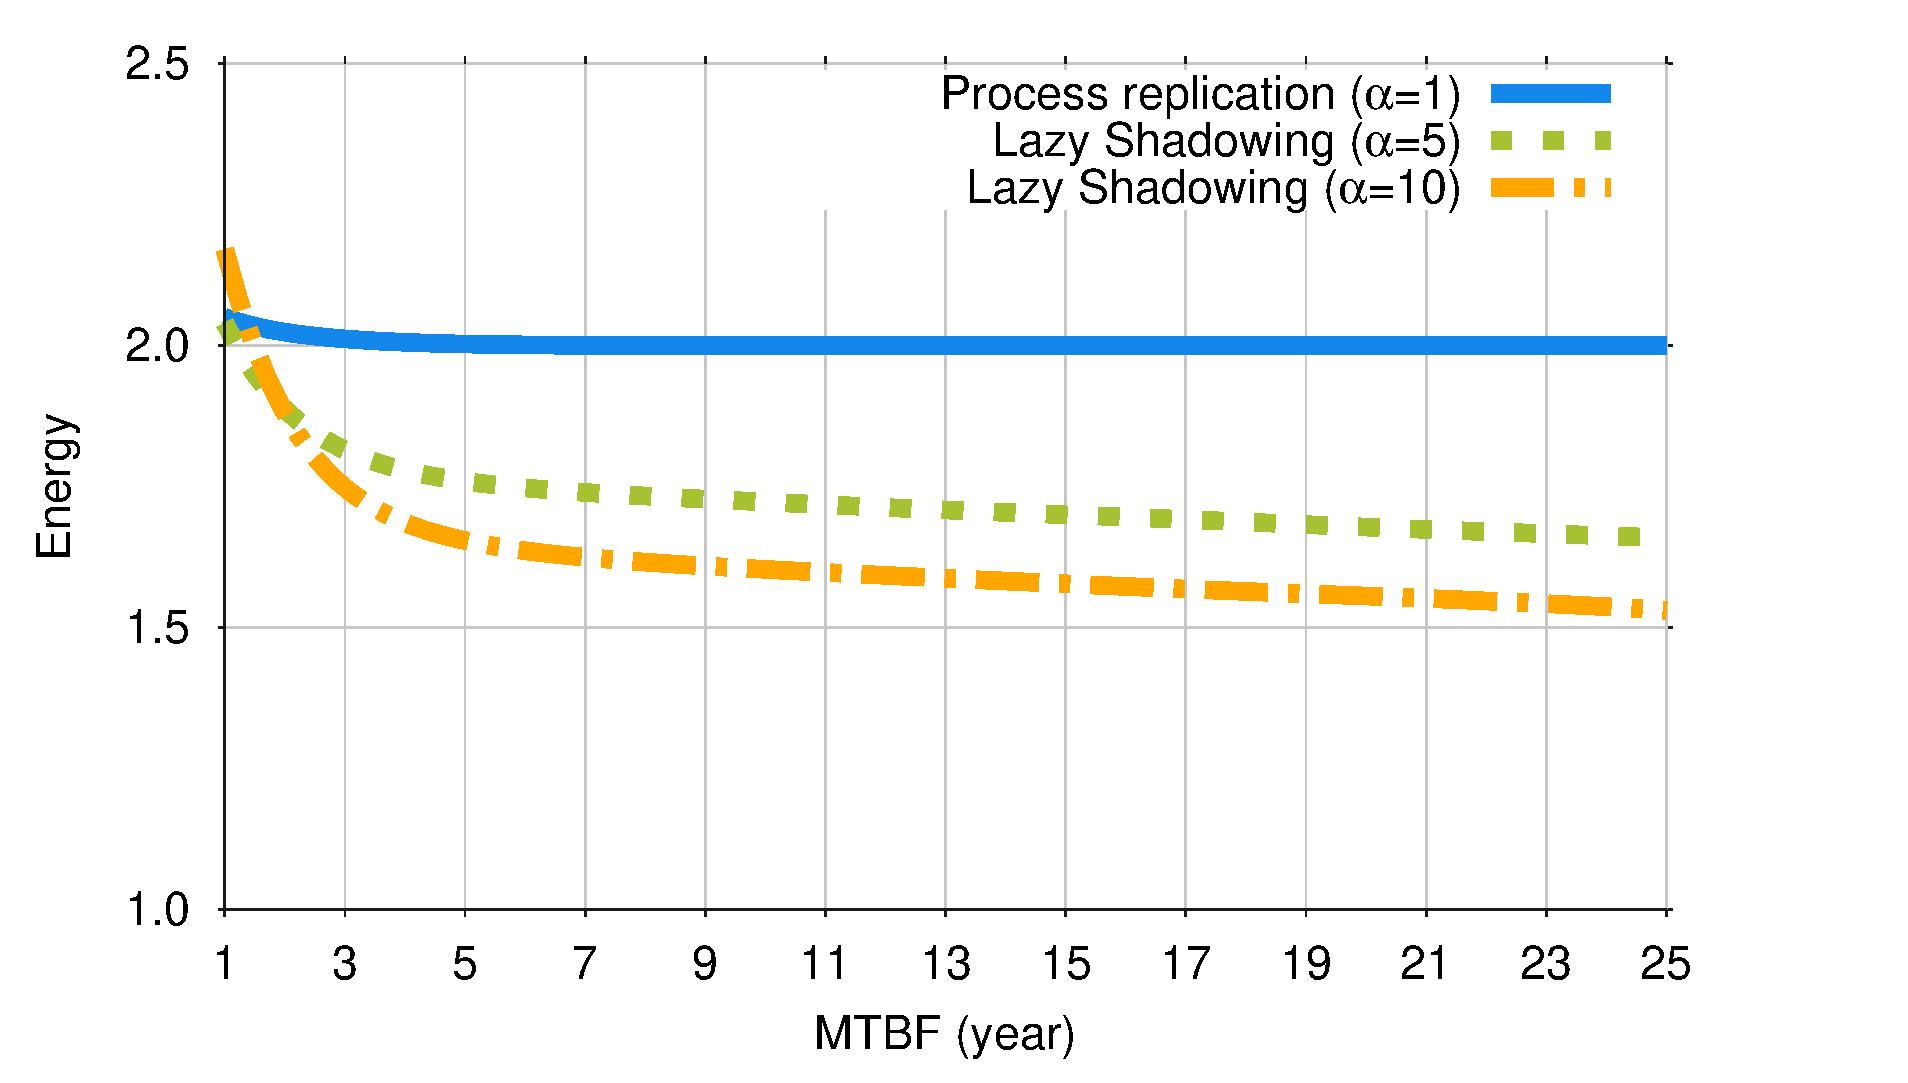
\includegraphics[width=0.7\columnwidth]{Figures/gen_energy.eps}
			%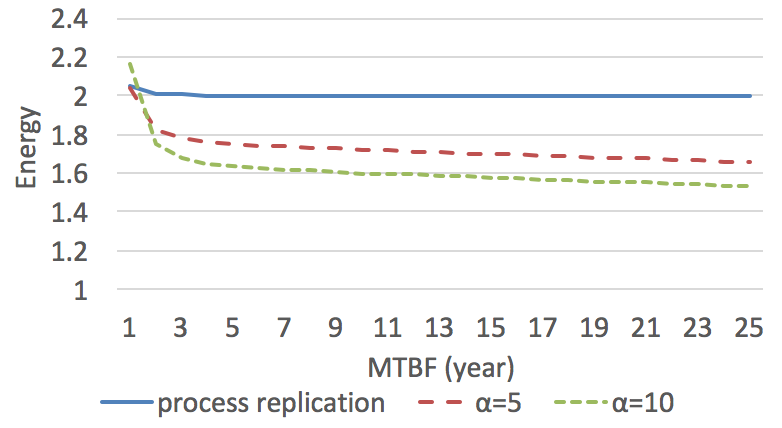
\includegraphics[width=0.7\columnwidth]{Figures/te32}
		} 
	\end{center}
	%\vskip -0.22in 
	\caption{Comparison of completion time and energy consumption. $W=10^6$ hours, $N=10^6$, $\rho=0.5$.}
	\label{fig:3}
\end{figure}

%By definition, the application fatal failure probability for checkpointing is 0, as it periodically saves the execution states, from which the computation can be resumed upon failure. Figure~\ref{fig:f3} shows that due to collocation, the application fatal failure probability increases for Lazy Shadowing. 
We had a comprehensive study of the application fatal failure probabilities using models in Section~\ref{anal_app_fail}. Results show that application fatal failure probability increases slightly for Lazy Shadowing compared to process replication, as a result of shadow collocation (discussed in Section~\ref{sec:leaping_shadows}). However, even with unrealistically low MTBF of 1 year, Lazy Shadowing is still able to complete without rollback with greater than 0.75 probability. Therefore, we will not further discuss application fatal failure probability.  


%It is clear from Figure~\ref{fig:t31} that checkpointing incurs significant delay, indicating that it may not be a viable fault tolerance approach for future extreme-scale computing. 
Our results show that at extreme-scale, the completion time and energy consumption of checkpointing are orders of magnitude larger than those of Lazy Shadowing and process replication. Thus, we choose not to plot a separate graph for checkpointing in the interest of space. 
%so large that the comparison between process replication and Lazy Shadowing is invisible. Therefore, we re-plot the comparison between Lazy Shadowing and process replication in Figure~\ref{fig:t32} and~\ref{fig:e32}, with checkpointing removed. 
Figure~\ref{fig:t32} reveals that the most time efficient choice largely depends on MTBF. 
%More specifically, process replication consumes less time when MTBF is low while otherwise Lazy Shadowing is more efficient.
When MTBF is high, Lazy Shadowing requires less time as more cores are used for main processes and less workload is assigned to each process. As MTBF decreases, process replication outperforms Lazy Shadowing as a result of the increased likelyhood of rollback for Lazy Shadowing.
%This is because of the increased probability of re-execution for Lazy Shadowing when failure rate is high. 
In terms of energy consumption, Lazy Shadowing has much more advantage over process replication. For MTBF from 2 to 25 years, Lazy Shadowing with $\alpha=5$ can achieve 9.6-17.1\% energy saving, while the saving increases to 13.1- 23.3\% for $\alpha=10$. The only exception is when MTBF is extremely low (1 year), Lazy Shadowing with $\alpha=10$ consumes more energy because of extended execution time.








\subsection{Impact of the number of cores}
\label{eval_core}
The system scale, measured in number of cores, has a direct impact on the failure rate seen by the application. To study its impact, we varies $N$ from 10,000 to 1,000,000 with $W$ scaled proportionally, i.e., $W=N$. When MTBF is 5 years, the results are shown in Figure~\ref{fig:n5}. Please note that the time and energy for checkpointing when $N=1,000,000$ are beyond the scope of the figures, so we mark their values on top of their columns. When completion time is considered, Figure~\ref{fig:nt5} clearly shows that each of the three fault tolerance alternatives has its own advantage. Specifically, checkpointing is the best choice for small systems with around 10,000 cores, Lazy Shadowing outperforms others for systems with around 100,000 cores, while process replication has slight advantage over Lazy Shadowing for larger systems. On the other hand, Lazy Shadowing wins for all system sizes covered in Figure~\ref{fig:ne5}, when energy consumption is considered. The comparison is different when MTBF is 25 years, as shown in Figure~\ref{fig:n25}. Though improved to a large extent, the performance of checkpointing is still much worse than that of the other two approaches when $N$ is 1,000,000. Lazy Shadowing also benefits from the increased MTBF, and further reduces its completion time and energy consumption for system sizes. In addition, Lazy Shadowing is able to achieve shorter completion time than process replication when $N$ reaches 1,000,000.

\begin{figure}[!t]
	\begin{center}
		\subfigure[Expected completion time]
		{
			\label{fig:nt5}
			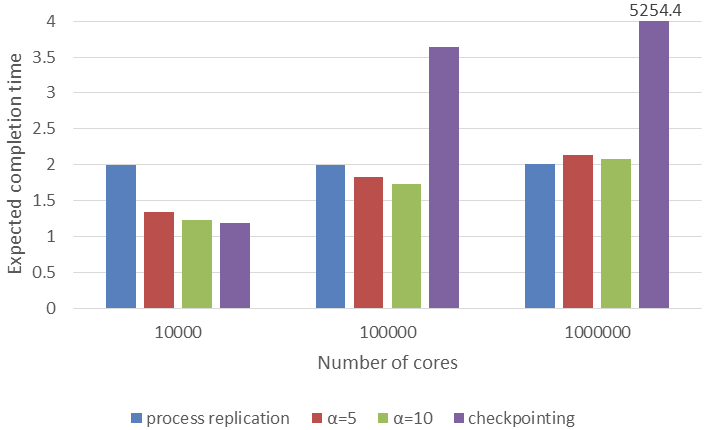
\includegraphics[width=\columnwidth]{Figures/nt5}
		} 
		\subfigure[Expected energy consumption]
		{
			\label{fig:ne5}
			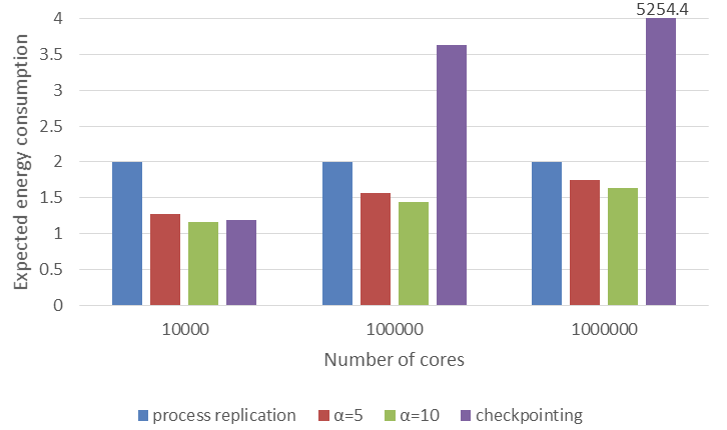
\includegraphics[width=\columnwidth]{Figures/ne5}
		} 
	\end{center}
	%\vskip -0.22in 
	\caption{Sensitivity to number of cores. $W=N$, MTBF=5 years, $\rho=0.5$.}
	\label{fig:n5}
\end{figure}

\begin{figure}[!t]
	\begin{center}
		\subfigure[Expected completion time]
		{
			\label{fig:nt25}
			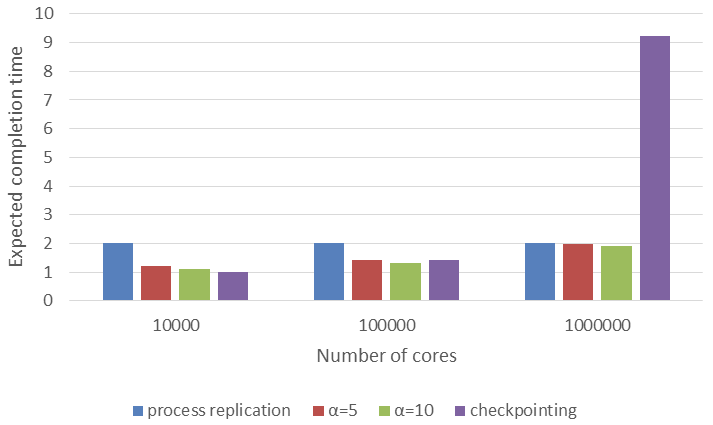
\includegraphics[width=\columnwidth]{Figures/nt25}
		} 
		\subfigure[Expected energy consumption]
		{
			\label{fig:ne25}
			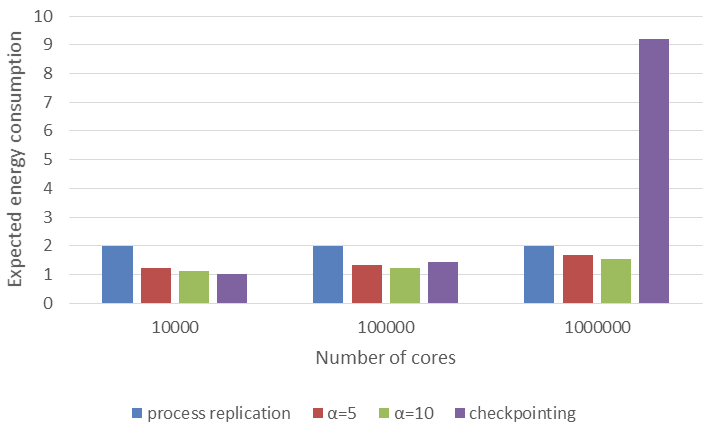
\includegraphics[width=\columnwidth]{Figures/ne25}
		} 
	\end{center}
	%\vskip -0.22in 
	\caption{Sensitivity to number of cores. $W=N$, MTBF=25years, $\rho=0.5$.}
	\label{fig:n25}
\end{figure}


\subsection{Impact of workload}
\label{eval_workload}
To a large extent, workload determines the time exposed to failures. With other factors being the same, an application with a larger workload is likely to encounter more failures during its execution. %Hence, it is intuitive that workload would impact the performance comparison. 
Fixing $N$ at 1,000,000, we increase $W$ from 1,000,000 hours to 12,000,000 hours. Figure~\ref{fig:w25} assumes a MTBF of 25 years and shows both the time and energy. Checkpointing has the worst performance in all cases. In terms of completion time, process replication is more efficient when workload reaches 6,000,000 hours. Considering energy consumption, however, Lazy Shadowing is able to achieve the most saving in all cases. %When MTBF of 5 years is used, the difference is that process replication consumes less energy than Lazy Shadowing when $W$ reaches 6,000,000.

\begin{figure}[!t]
	\begin{center}
		\subfigure[Expected completion time]
		{
			\label{fig:wt25}
			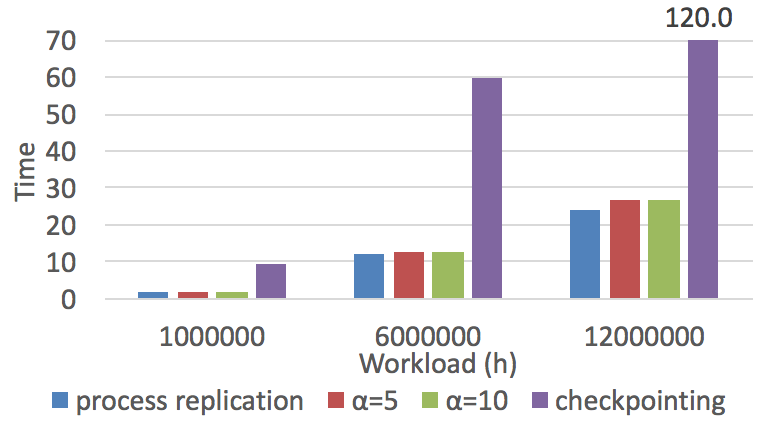
\includegraphics[width=0.7\columnwidth]{Figures/twt25}
		} 
		\subfigure[Expected energy consumption]
		{
			\label{fig:we25}
			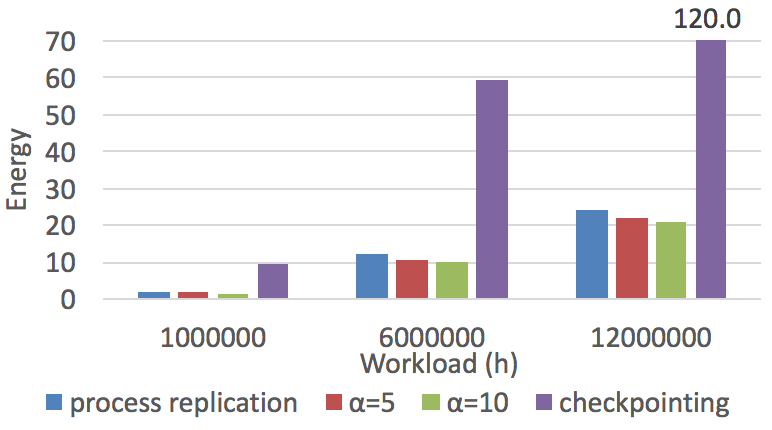
\includegraphics[width=0.7\columnwidth]{Figures/twe25}
		} 
	\end{center}
	\vskip -0.04in 
	\caption{Sensitivity to workload. $N=10^6$, MTBF=25 years, $\rho=0.5$.}
	\label{fig:w25}
\end{figure}


\subsection{Impact of static power ratio}
\label{eval_static_power}
With various architectures and organizations, servers
vary in terms of
power consumption. The static power ratio $\rho$ is used to abstract the
amount of static power consumed versus dynamic power. 
%$\rho$ does not impact the completion time, but power and energy consumption.
Considering modern systems, we vary $\rho$ from 0.3 to 0.7 and study its effect
on the expected energy consumption. The results for Lazy Shadowing with $\alpha=5$ are normalized to that of process replication and shown in 
Figure~\ref{fig:power_ratio}. The results for other values of $\alpha$ have similar behavior and thus are not shown. Lazy Shadowing achieves
more energy saving when static power ratio is low, since it saves dynamic 
power but not static power. When static power ratio is low ($\rho=0.3$), Lazy Shadowing
is able to save 20\%-24\% energy for the MTBF of 5 to 25 years. The saving decreases to 5\%-11\% when $\rho$ reaches 0.7. 

\begin{figure}[!t]
	\begin{center}
		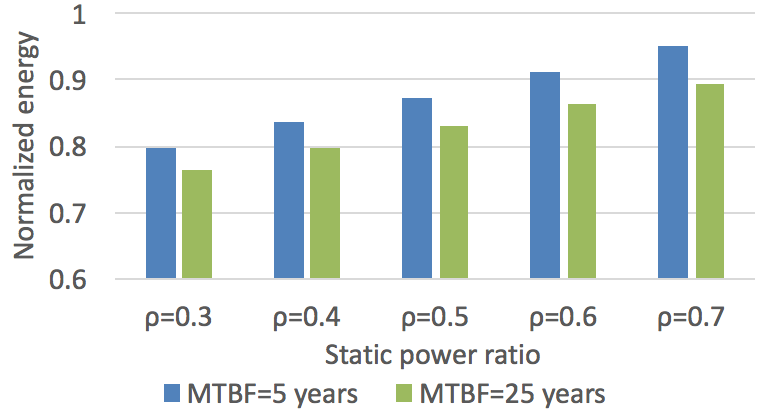
\includegraphics[width=0.7\columnwidth]{Figures/ts_power_5}
	\end{center}
	%\vskip -0.22in 
	\caption{Impact of static power ratio on energy consumption. $W=10^6$ hours, $N=10^6$, $\alpha$=5.}
	\label{fig:power_ratio}
\end{figure}


\subsection{Adding collocation overhead}
\label{eval_collocation}
%The last study is conducted to capture the impact on the 
%performance of Lazy Shadowing brought by 
%collocation overhead. We re-model the speed of shadows as $\sigma_s^b=\frac{1}{\alpha^{1.5}}$ to simulate the 
%effect of memory thrashing and context switch. 

Lazy Shadowing increases memory requirement\footnote{Note that this problem is not intrinsic to Lazy Shadowing, as in-memory checkpointing also requires extra memory.} when multiple shadows are collocated. Moreover, this may have an impact on the execution rate of the shadows due to cache contention and context switch. 
To capture this effect,  
we re-model the rate of shadows as $\sigma_s^b=\frac{1}{\alpha^{1.5}}$.
Figure~\ref{fig:comp_vary_fail_speed} shows the impact of collocation overhead on expected energy consumption for Lazy Shadowing with $\alpha=5$, with all the values normalized to that of process replication. The results for other values of $\alpha$ have similar behavior and thus are not shown. As expected, energy consumption is penalized because
of slowing down of the shadows. It is surprising, however, that the impact is quite small, with the largest difference being 4.4\%. The reason is that shadow leaping can take advantage of the recovery time after each failure and achieve forward progress for shadow processes that fall behind. When $\alpha=10$, the largest difference further decreases to 2.5\%. 

%As expected, both completion time and energy consumption are penalized because
%of slowing down of the shadows. It is surprising, however, that Lazy Shadowing with $\alpha=3$ is impacted by the 
%most, while when $\alpha=9$, which means collocating more shadows on each shadow core, is slightly influenced. After careful analysis,
%we realize that the reason is $\alpha=3$ had the largest values for completion time and energy consumption. Even the percentage of increase after adding the penalty is the smallest, the absolute increase is still the largest. 
%When $\alpha=9$, Lazy Shadowing can still achieve 15\%-20\% energy saving with less than 7\% increase in completion time. 

\begin{figure}[t]
	\begin{center}
		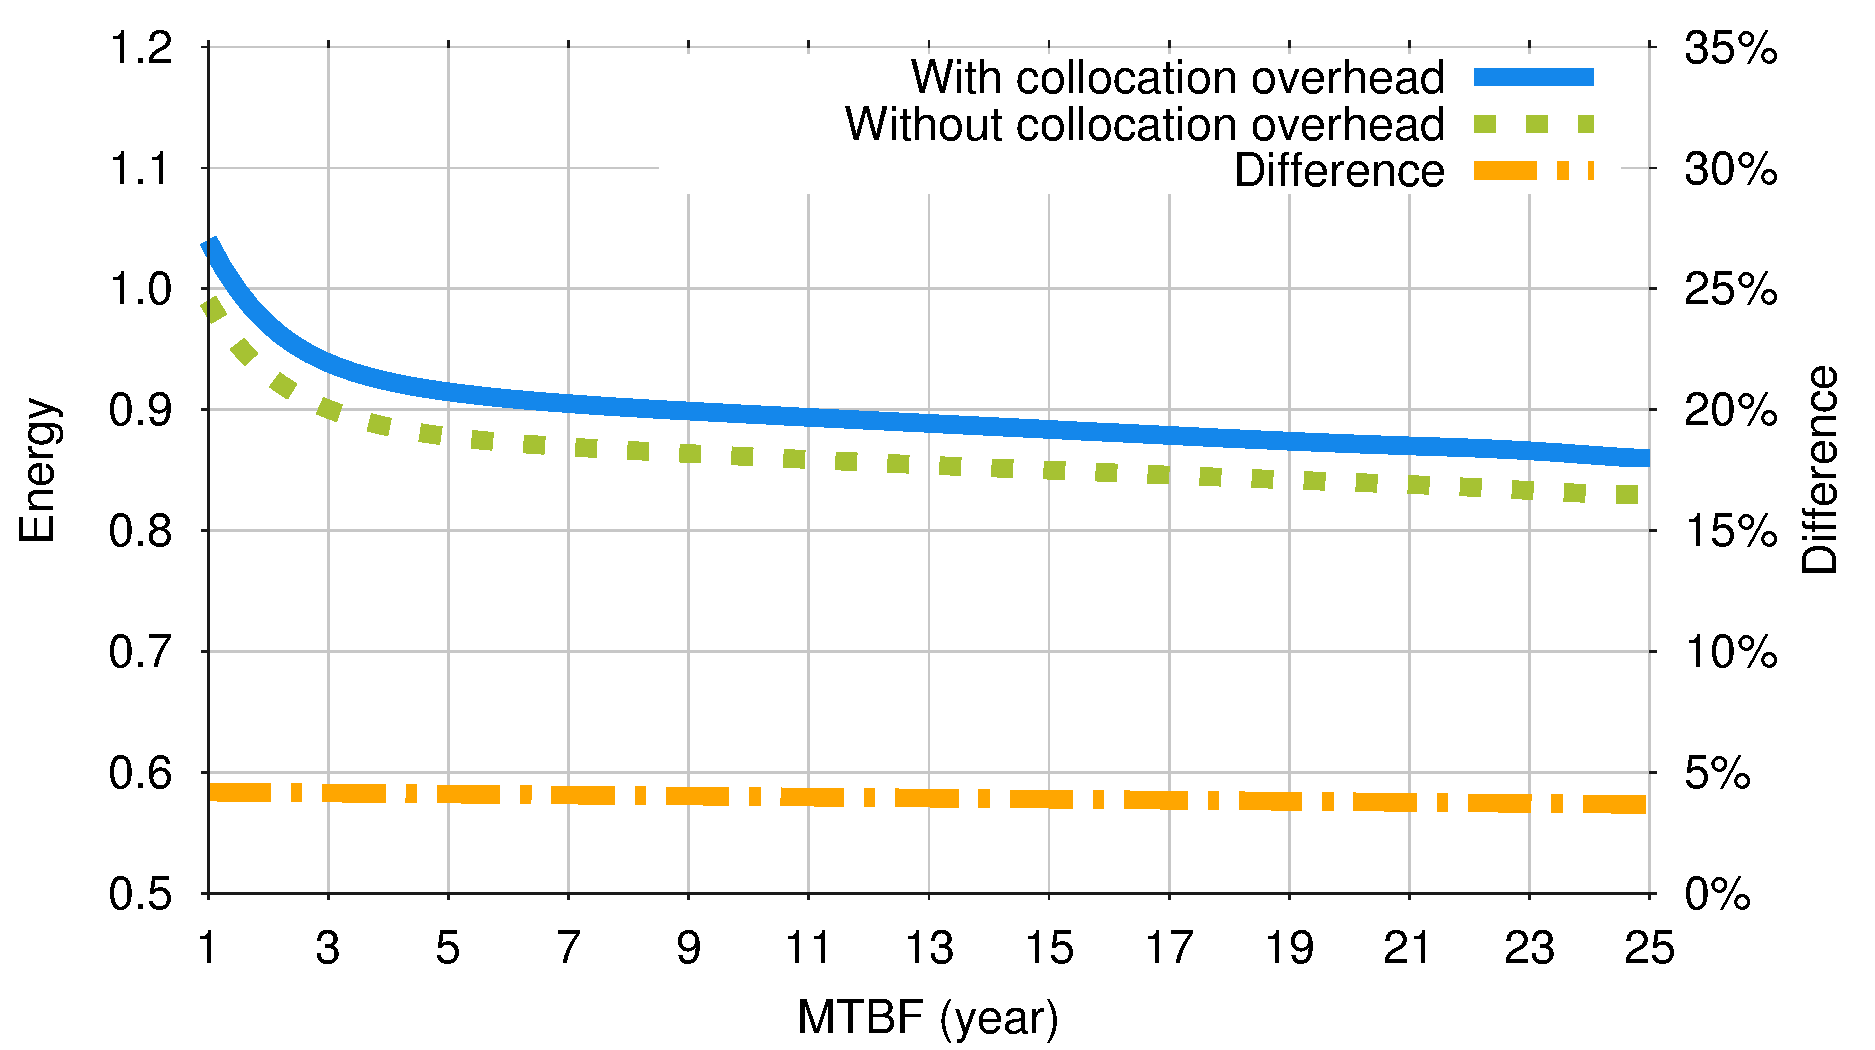
\includegraphics[width=0.7\columnwidth]{Figures/collocation.pdf}
		%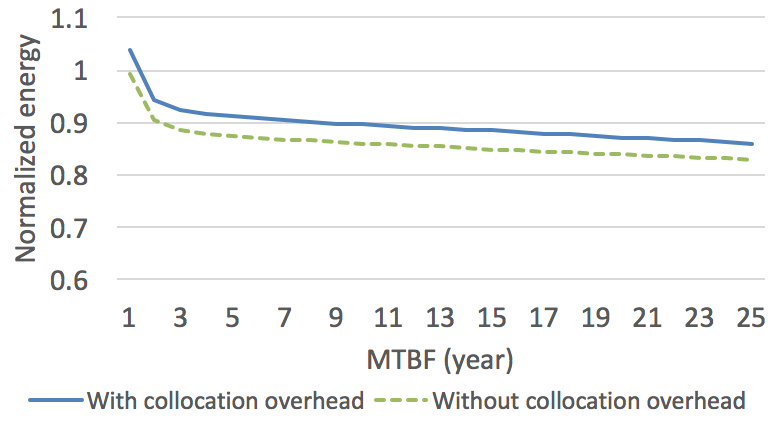
\includegraphics[width=0.7\columnwidth]{Figures/tcollocation}
	\end{center}
	%\vskip -0.22in 
	\caption{Impact of collocation overhead on energy consumption. $W=10^6$ hours, $N=10^6$, $\rho$=0.5, $\alpha$=5.}
	\label{fig:comp_vary_fail_speed}
\end{figure}

